


\documentclass{article}

\usepackage[pdftex]{graphicx}
\graphicspath {{figures/}}			 % Used to insert images from the figures folder (relative path)

\usepackage{amsmath, amsthm, amssymb} % assumes amsmath package installed
\usepackage{hyperref} 				 % Insert hyperlinks 
\setlength{\parindent}{0pt}			 % Remove the automatic indent for new paragraphs

\usepackage[T1]{fontenc}
\usepackage{titling}

\setlength{\droptitle}{-8em}   % This is your set screw

\title{Laser Scanner Transforms}
\author{Brendan Emery}
\date{February 2016}



\begin{document}
\maketitle

\begin{abstract}
\noindent In this document I outline the relative transforms used on the laser scanning box and how they're calculated/implemented. The final goal is to find the roll and pitch of the of the robot relative to it's stabilised frame, i.e. $ {^{base\_stabilised}R\ _{base\_link}} $. This transform is broadcasted and used to transform the incoming laser scans used for localisation and mapping. Refer to \url{<http://wiki.ros.org/hectoR\ _slam/Tutorials/SettingUpForYourRobot>} for a description of the coordinate frame system that I have used. In addition to the standard frames described above, I have also added an imu\_corrected frame. This frame will give the imu values corrected by the initial offset of the imu due to any unknown rotations between the IMU and the robot that have not been accounted for in the urdf file. There is also an inertial frame which is determined by the IMU.
\end{abstract}

\vspace*{1cm}

% Your image goes here
\noindent
\makebox[\textwidth]{
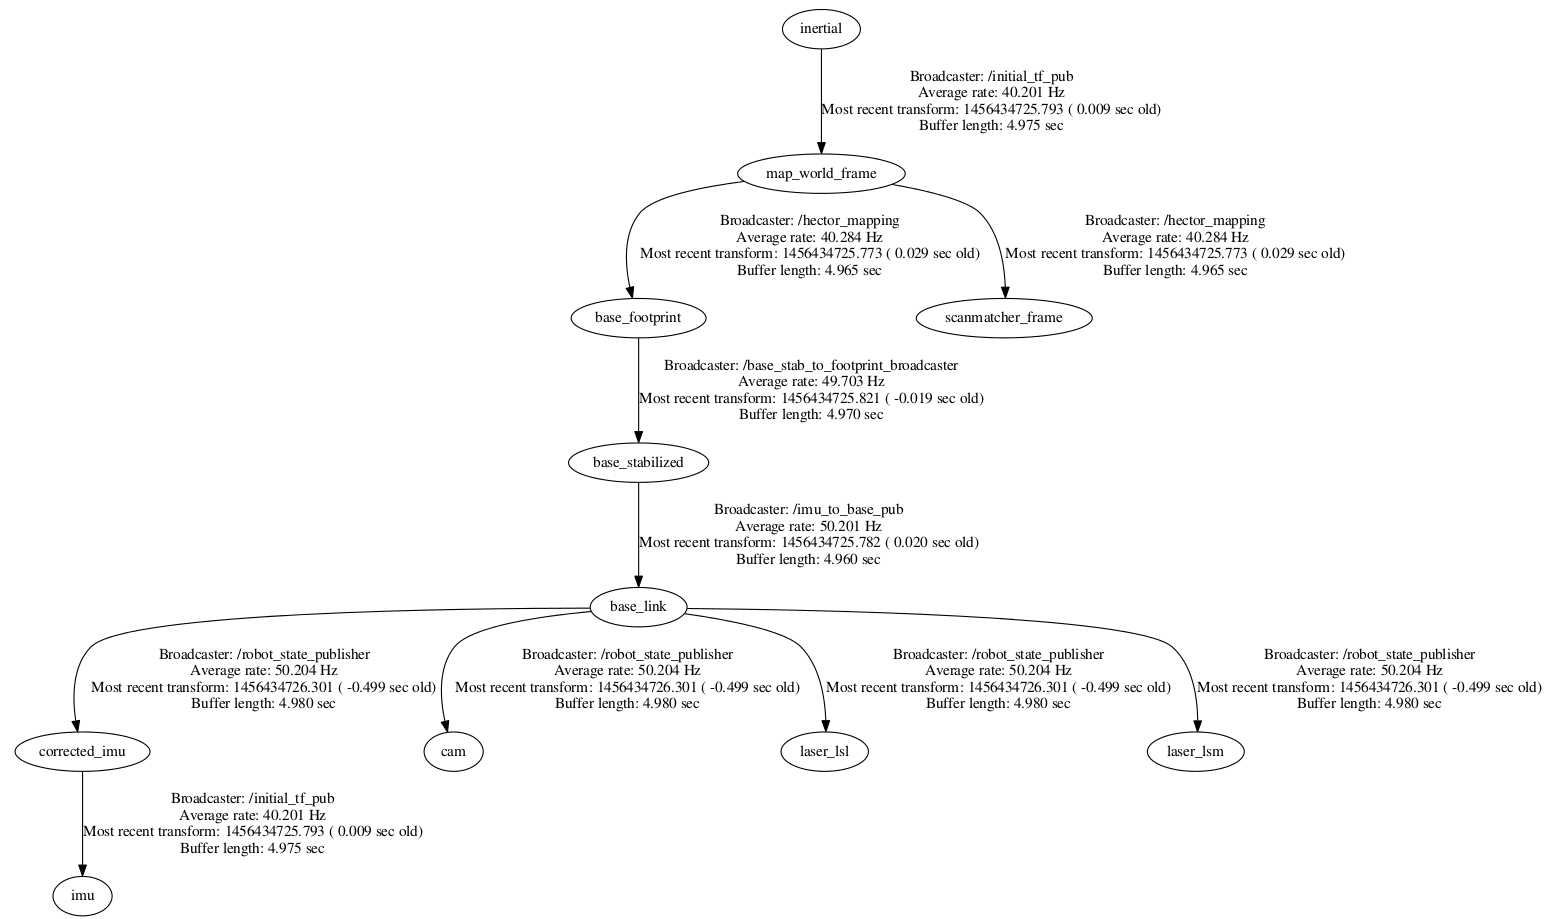
\includegraphics[scale=0.31]{frame_diagram}
}
%

\vspace*{0cm}

%\begin{figure}[h!]
% \centering
  %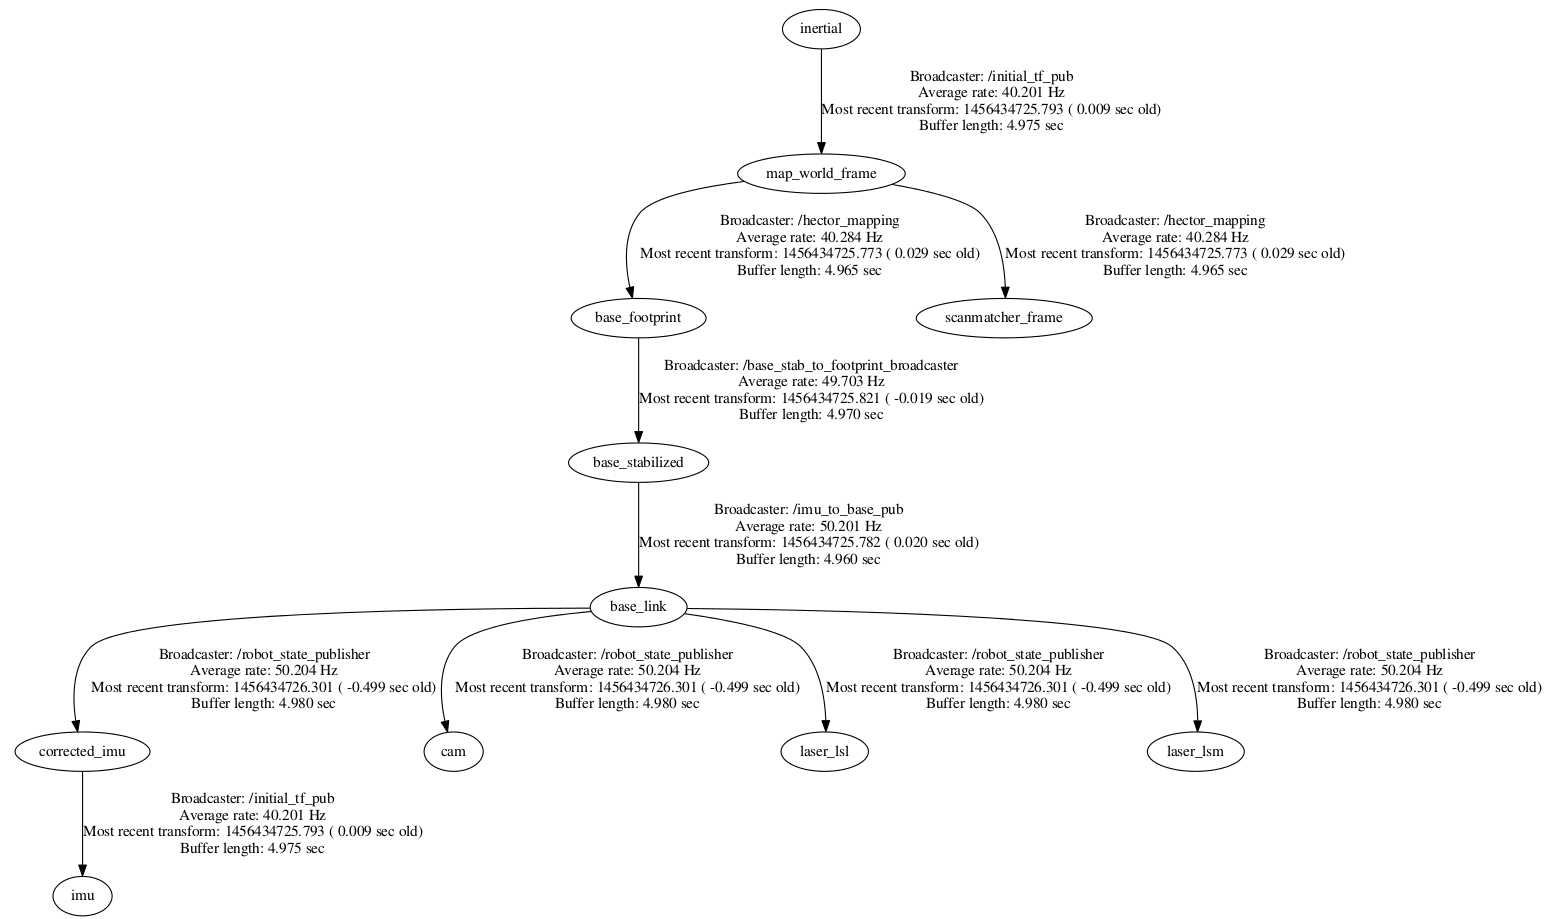
\includegraphics[width=1.1\textwidth]{frame_diagram}
%  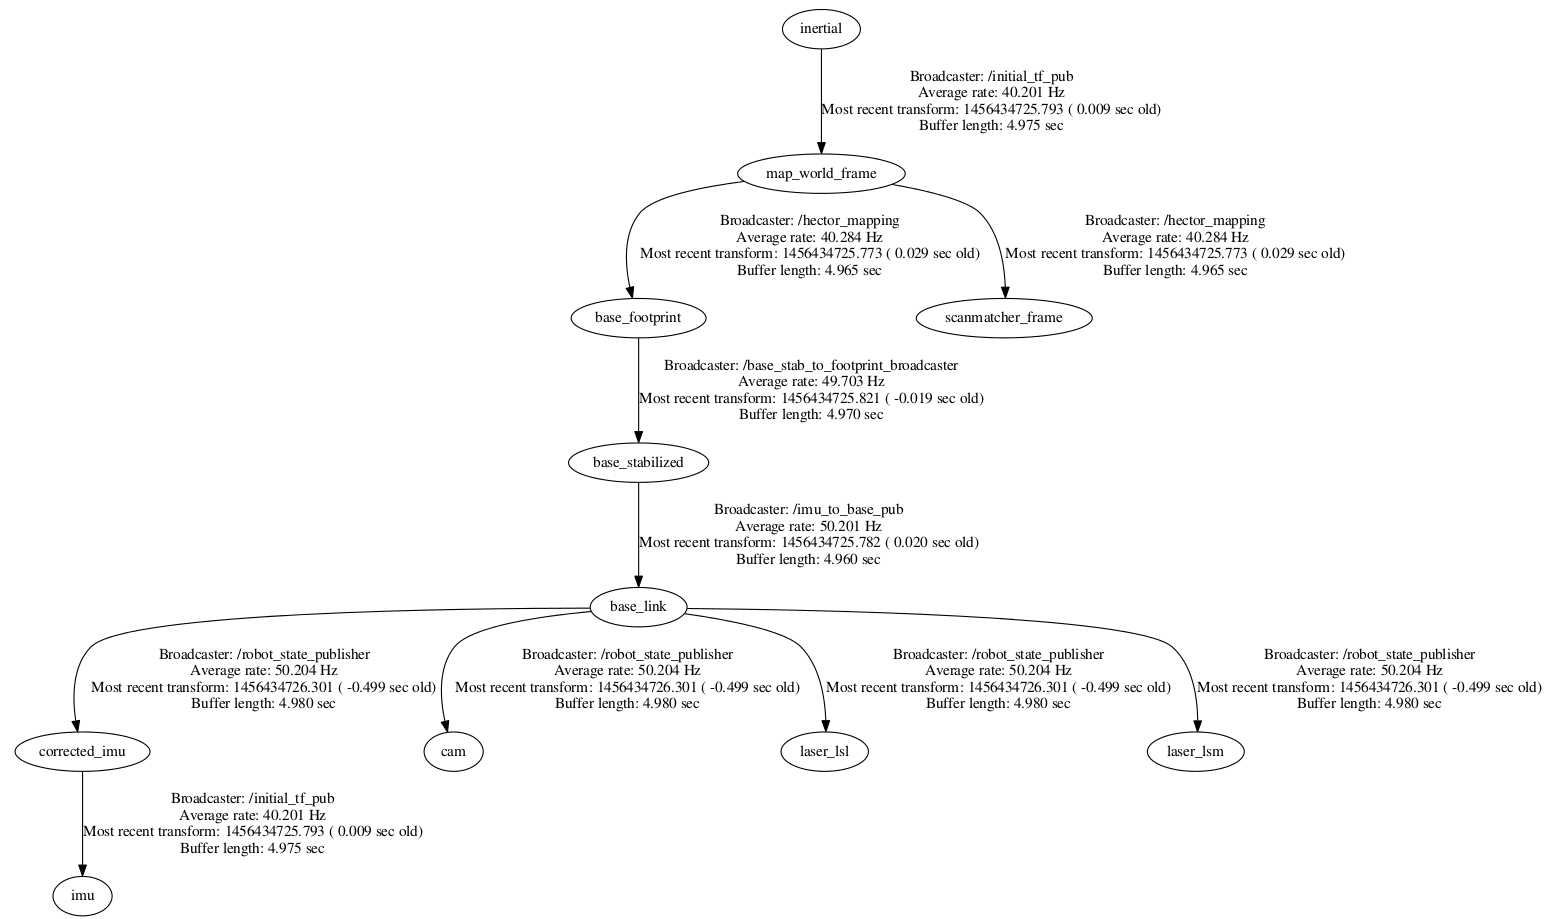
\includegraphics[scale=0.3]{frame_diagram}
% \caption{Coordinate frame system used}
% \end{figure}

\section{Find initial transforms}

\subsection{Static transform: URDF file}
The user must update the urdf file to give the transform $ {^{corrected\_imu}R\ _{base\_link}} $. This transform is the rotation between the base\_link of the robot and the coordinate frame of the IMU as it sits on the robot. This is done inside "data\_recorder/urdf/laser\_scanner\_description.urdf".

\subsection{Find Initial IMU Offset}
At time t=0, the user should power up the unit on flat ground. To account for any angular offsets that haven't been accounted for in the transform between the imu and base\_link, we provide a transform between the imu and the corrected imu frame:
\begin{equation}
^{corrected\_imu}R\ _{imu} =\ (^{I}R\ _{corrected\_imu})^T \times\  ^{I}R\ _{imu}
\end{equation}

where,
\begin{equation}
^{I}R\ _{imu} =\ R\ _z(\alpha_0) \times\  R\ _y(\beta_0) \times\  R\ _x(\gamma_0) 
\end{equation}

where $\gamma_0$ =\ roll, $\beta_0$ =\ pitch and $\alpha_0$ =\ yaw of the imu in the inertial frame at t=0 and $^{I}R\ _{corrected\_imu} $ is the transform between the current IMU position on the robot and the inertial frame given in the IMU datasheet. 
\\

The user will provide the static roll, pitch and yaw values giving the offset of the imu in the inertial frame at t=0. However, since the yaw value from the IMU updates slowly, applying the initial yaw value as an offset can cause issues. So when we offset the IMU reading by applying $^{corrected\_imu}R\ _{imu}$, we only want to offset the roll and pitch. Therefore, we will add the IMU's yaw value to the static offset determined above to give:

\begin{equation}
^{I}R\ _{corrected\_imu} = R\ _z(\alpha_0\ +\ \alpha_{static}) \times\  R\ _y(\beta_{static}) \times\  R\ _x(\gamma_{static})
\end{equation}

We can now apply this transform to the IMU messages to get roll and pitch offset-corrected IMU messages. This is done inside "data\_recorder/src/initial\_tf\_pub.cpp"


\subsection{Static transform: static publisher}
The user must use a static\_broadcaster\_publisher to provide $ {^{I}R\ _{map}}$. This is done inside "data\_recorder/launch/data\_recorder.launch" The map frame is provided by the hector mapping package and will be initialised to be aligned and coincident with the base\_footprint frame (which is also aligned with the base\_link frame at t=0). Therefore the rotation between the inertial and map frame will be given by:

\begin{equation}
^{I}R\ _{map}=\ ^{I}R\ _{base\_link},\ when\ t=0
\end{equation}

Therefore,

\begin{equation}
^{I}R\ _{map}=\ ^{I}R\ _{base\_link}=\ ^{I}R\ _{corrected\_imu} \times\ ^{corrected\_imu}R\ _{base\_link},\ when\ t=0
\end{equation}

The user needs to then manually determine these two transforms and then calculate and publish $^{I}R\ _{map}$. This is done inside "data\_recorder/src/initial\_tf\_pub.cpp"



\section{Find Robot Orientation}
We want to find the base\_link with respect to the base\_stabilised frame at any time to give the roll and pitch values of the robot.
\\

At any time, the corrected IMU values can be given by:
\begin{equation}
^{I}R\ _{corrected\_imu} =\ ^{I}R\ _{imu} \times\  (^{corrected\_imu}R\ _{imu})^T\\
\end{equation}
\begin{align}
^{I}R\ _{base\_link} & =\ ^{I}R\ _{corrected\_imu} \times\  ^{corrected\_imu}R\ _{base\_link}\\
\end{align}

Therefore,
\begin{align}
^{map}R\ _{base\_link} & =\ (^{I}R\ _{map})^T \times\  ^{I}R\ _{base\_link}\\
 & =\ \ R\ _z(\alpha) \times\  R\ _y(\beta) \times\  R\ _x(\gamma) 
\end{align}

where $\gamma$ =\ roll, $\beta$ =\ pitch and $\alpha$ =\ yaw of the robot in the map frame.\\

Since the base\_link and base\_stabilised frames have the same heading (i.e. their yaw value with respect to the map is the same) and the base\_stabilised frame has roll =\ pitch =\ 0:

\begin{equation}
^{map}R\ _{base\_stabilised} =\ R\ _z(\alpha) 
\end{equation}

So,
\begin{align}
^{I}R\ _{base\_stabilised} & =\ ^{I}R\ _{map} \times\  ^{map}R\ _{base\_stabilised}\\
 & =\ ^{I}R\ _{map} \times\  R\ _z(\alpha) 
\end{align}

Therefore,
\begin{align}
^{base\_stabilised}R\ _{base\_link} &=\ (^{I}R\ _{base\_stabilised})^T \times\  ^{I}R\ _{base\_link}\\
 &\ = (^{I}R\ _{map} \times\  R_z(\alpha))^T \times\  R\ _z(\alpha) \times\  R\ _y(\beta) \times\  R\ _x(\gamma) 
\end{align}

This is done inside "data\_recorder/src/imu\_to\_base\_pub.cpp"


\end{document}
